% Options for packages loaded elsewhere
\PassOptionsToPackage{unicode}{hyperref}
\PassOptionsToPackage{hyphens}{url}
%
\documentclass[
]{article}
\usepackage{amsmath,amssymb}
\usepackage{iftex}
\ifPDFTeX
  \usepackage[T1]{fontenc}
  \usepackage[utf8]{inputenc}
  \usepackage{textcomp} % provide euro and other symbols
\else % if luatex or xetex
  \usepackage{unicode-math} % this also loads fontspec
  \defaultfontfeatures{Scale=MatchLowercase}
  \defaultfontfeatures[\rmfamily]{Ligatures=TeX,Scale=1}
\fi
\usepackage{lmodern}
\ifPDFTeX\else
  % xetex/luatex font selection
\fi
% Use upquote if available, for straight quotes in verbatim environments
\IfFileExists{upquote.sty}{\usepackage{upquote}}{}
\IfFileExists{microtype.sty}{% use microtype if available
  \usepackage[]{microtype}
  \UseMicrotypeSet[protrusion]{basicmath} % disable protrusion for tt fonts
}{}
\makeatletter
\@ifundefined{KOMAClassName}{% if non-KOMA class
  \IfFileExists{parskip.sty}{%
    \usepackage{parskip}
  }{% else
    \setlength{\parindent}{0pt}
    \setlength{\parskip}{6pt plus 2pt minus 1pt}}
}{% if KOMA class
  \KOMAoptions{parskip=half}}
\makeatother
\usepackage{xcolor}
\usepackage[margin=1in]{geometry}
\usepackage{color}
\usepackage{fancyvrb}
\newcommand{\VerbBar}{|}
\newcommand{\VERB}{\Verb[commandchars=\\\{\}]}
\DefineVerbatimEnvironment{Highlighting}{Verbatim}{commandchars=\\\{\}}
% Add ',fontsize=\small' for more characters per line
\usepackage{framed}
\definecolor{shadecolor}{RGB}{248,248,248}
\newenvironment{Shaded}{\begin{snugshade}}{\end{snugshade}}
\newcommand{\AlertTok}[1]{\textcolor[rgb]{0.94,0.16,0.16}{#1}}
\newcommand{\AnnotationTok}[1]{\textcolor[rgb]{0.56,0.35,0.01}{\textbf{\textit{#1}}}}
\newcommand{\AttributeTok}[1]{\textcolor[rgb]{0.13,0.29,0.53}{#1}}
\newcommand{\BaseNTok}[1]{\textcolor[rgb]{0.00,0.00,0.81}{#1}}
\newcommand{\BuiltInTok}[1]{#1}
\newcommand{\CharTok}[1]{\textcolor[rgb]{0.31,0.60,0.02}{#1}}
\newcommand{\CommentTok}[1]{\textcolor[rgb]{0.56,0.35,0.01}{\textit{#1}}}
\newcommand{\CommentVarTok}[1]{\textcolor[rgb]{0.56,0.35,0.01}{\textbf{\textit{#1}}}}
\newcommand{\ConstantTok}[1]{\textcolor[rgb]{0.56,0.35,0.01}{#1}}
\newcommand{\ControlFlowTok}[1]{\textcolor[rgb]{0.13,0.29,0.53}{\textbf{#1}}}
\newcommand{\DataTypeTok}[1]{\textcolor[rgb]{0.13,0.29,0.53}{#1}}
\newcommand{\DecValTok}[1]{\textcolor[rgb]{0.00,0.00,0.81}{#1}}
\newcommand{\DocumentationTok}[1]{\textcolor[rgb]{0.56,0.35,0.01}{\textbf{\textit{#1}}}}
\newcommand{\ErrorTok}[1]{\textcolor[rgb]{0.64,0.00,0.00}{\textbf{#1}}}
\newcommand{\ExtensionTok}[1]{#1}
\newcommand{\FloatTok}[1]{\textcolor[rgb]{0.00,0.00,0.81}{#1}}
\newcommand{\FunctionTok}[1]{\textcolor[rgb]{0.13,0.29,0.53}{\textbf{#1}}}
\newcommand{\ImportTok}[1]{#1}
\newcommand{\InformationTok}[1]{\textcolor[rgb]{0.56,0.35,0.01}{\textbf{\textit{#1}}}}
\newcommand{\KeywordTok}[1]{\textcolor[rgb]{0.13,0.29,0.53}{\textbf{#1}}}
\newcommand{\NormalTok}[1]{#1}
\newcommand{\OperatorTok}[1]{\textcolor[rgb]{0.81,0.36,0.00}{\textbf{#1}}}
\newcommand{\OtherTok}[1]{\textcolor[rgb]{0.56,0.35,0.01}{#1}}
\newcommand{\PreprocessorTok}[1]{\textcolor[rgb]{0.56,0.35,0.01}{\textit{#1}}}
\newcommand{\RegionMarkerTok}[1]{#1}
\newcommand{\SpecialCharTok}[1]{\textcolor[rgb]{0.81,0.36,0.00}{\textbf{#1}}}
\newcommand{\SpecialStringTok}[1]{\textcolor[rgb]{0.31,0.60,0.02}{#1}}
\newcommand{\StringTok}[1]{\textcolor[rgb]{0.31,0.60,0.02}{#1}}
\newcommand{\VariableTok}[1]{\textcolor[rgb]{0.00,0.00,0.00}{#1}}
\newcommand{\VerbatimStringTok}[1]{\textcolor[rgb]{0.31,0.60,0.02}{#1}}
\newcommand{\WarningTok}[1]{\textcolor[rgb]{0.56,0.35,0.01}{\textbf{\textit{#1}}}}
\usepackage{graphicx}
\makeatletter
\def\maxwidth{\ifdim\Gin@nat@width>\linewidth\linewidth\else\Gin@nat@width\fi}
\def\maxheight{\ifdim\Gin@nat@height>\textheight\textheight\else\Gin@nat@height\fi}
\makeatother
% Scale images if necessary, so that they will not overflow the page
% margins by default, and it is still possible to overwrite the defaults
% using explicit options in \includegraphics[width, height, ...]{}
\setkeys{Gin}{width=\maxwidth,height=\maxheight,keepaspectratio}
% Set default figure placement to htbp
\makeatletter
\def\fps@figure{htbp}
\makeatother
\setlength{\emergencystretch}{3em} % prevent overfull lines
\providecommand{\tightlist}{%
  \setlength{\itemsep}{0pt}\setlength{\parskip}{0pt}}
\setcounter{secnumdepth}{-\maxdimen} % remove section numbering
<!--radix_placeholder_navigation_in_header-->
<meta name="distill:offset" content=""/>

<script type="application/javascript">

  window.headroom_prevent_pin = false;

  window.document.addEventListener("DOMContentLoaded", function (event) {

    // initialize headroom for banner
    var header = $('header').get(0);
    var headerHeight = header.offsetHeight;
    var headroom = new Headroom(header, {
      tolerance: 5,
      onPin : function() {
        if (window.headroom_prevent_pin) {
          window.headroom_prevent_pin = false;
          headroom.unpin();
        }
      }
    });
    headroom.init();
    if(window.location.hash)
      headroom.unpin();
    $(header).addClass('headroom--transition');

    // offset scroll location for banner on hash change
    // (see: https://github.com/WickyNilliams/headroom.js/issues/38)
    window.addEventListener("hashchange", function(event) {
      window.scrollTo(0, window.pageYOffset - (headerHeight + 25));
    });

    // responsive menu
    $('.distill-site-header').each(function(i, val) {
      var topnav = $(this);
      var toggle = topnav.find('.nav-toggle');
      toggle.on('click', function() {
        topnav.toggleClass('responsive');
      });
    });

    // nav dropdowns
    $('.nav-dropbtn').click(function(e) {
      $(this).next('.nav-dropdown-content').toggleClass('nav-dropdown-active');
      $(this).parent().siblings('.nav-dropdown')
         .children('.nav-dropdown-content').removeClass('nav-dropdown-active');
    });
    $("body").click(function(e){
      $('.nav-dropdown-content').removeClass('nav-dropdown-active');
    });
    $(".nav-dropdown").click(function(e){
      e.stopPropagation();
    });
  });
</script>

<style type="text/css">

/* Theme (user-documented overrideables for nav appearance) */

.distill-site-nav {
  color: rgba(255, 255, 255, 0.8);
  background-color: #0F2E3D;
  font-size: 15px;
  font-weight: 300;
}

.distill-site-nav a {
  color: inherit;
  text-decoration: none;
}

.distill-site-nav a:hover {
  color: white;
}

@media print {
  .distill-site-nav {
    display: none;
  }
}

.distill-site-header {

}

.distill-site-footer {

}


/* Site Header */

.distill-site-header {
  width: 100%;
  box-sizing: border-box;
  z-index: 3;
}

.distill-site-header .nav-left {
  display: inline-block;
  margin-left: 8px;
}

@media screen and (max-width: 768px) {
  .distill-site-header .nav-left {
    margin-left: 0;
  }
}


.distill-site-header .nav-right {
  float: right;
  margin-right: 8px;
}

.distill-site-header a,
.distill-site-header .title {
  display: inline-block;
  text-align: center;
  padding: 14px 10px 14px 10px;
}

.distill-site-header .title {
  font-size: 18px;
  min-width: 150px;
}

.distill-site-header .logo {
  padding: 0;
}

.distill-site-header .logo img {
  display: none;
  max-height: 20px;
  width: auto;
  margin-bottom: -4px;
}

.distill-site-header .nav-image img {
  max-height: 18px;
  width: auto;
  display: inline-block;
  margin-bottom: -3px;
}



@media screen and (min-width: 1000px) {
  .distill-site-header .logo img {
    display: inline-block;
  }
  .distill-site-header .nav-left {
    margin-left: 20px;
  }
  .distill-site-header .nav-right {
    margin-right: 20px;
  }
  .distill-site-header .title {
    padding-left: 12px;
  }
}


.distill-site-header .nav-toggle {
  display: none;
}

.nav-dropdown {
  display: inline-block;
  position: relative;
}

.nav-dropdown .nav-dropbtn {
  border: none;
  outline: none;
  color: rgba(255, 255, 255, 0.8);
  padding: 16px 10px;
  background-color: transparent;
  font-family: inherit;
  font-size: inherit;
  font-weight: inherit;
  margin: 0;
  margin-top: 1px;
  z-index: 2;
}

.nav-dropdown-content {
  display: none;
  position: absolute;
  background-color: white;
  min-width: 200px;
  border: 1px solid rgba(0,0,0,0.15);
  border-radius: 4px;
  box-shadow: 0px 8px 16px 0px rgba(0,0,0,0.1);
  z-index: 1;
  margin-top: 2px;
  white-space: nowrap;
  padding-top: 4px;
  padding-bottom: 4px;
}

.nav-dropdown-content hr {
  margin-top: 4px;
  margin-bottom: 4px;
  border: none;
  border-bottom: 1px solid rgba(0, 0, 0, 0.1);
}

.nav-dropdown-active {
  display: block;
}

.nav-dropdown-content a, .nav-dropdown-content .nav-dropdown-header {
  color: black;
  padding: 6px 24px;
  text-decoration: none;
  display: block;
  text-align: left;
}

.nav-dropdown-content .nav-dropdown-header {
  display: block;
  padding: 5px 24px;
  padding-bottom: 0;
  text-transform: uppercase;
  font-size: 14px;
  color: #999999;
  white-space: nowrap;
}

.nav-dropdown:hover .nav-dropbtn {
  color: white;
}

.nav-dropdown-content a:hover {
  background-color: #ddd;
  color: black;
}

.nav-right .nav-dropdown-content {
  margin-left: -45%;
  right: 0;
}

@media screen and (max-width: 768px) {
  .distill-site-header a, .distill-site-header .nav-dropdown  {display: none;}
  .distill-site-header a.nav-toggle {
    float: right;
    display: block;
  }
  .distill-site-header .title {
    margin-left: 0;
  }
  .distill-site-header .nav-right {
    margin-right: 0;
  }
  .distill-site-header {
    overflow: hidden;
  }
  .nav-right .nav-dropdown-content {
    margin-left: 0;
  }
}


@media screen and (max-width: 768px) {
  .distill-site-header.responsive {position: relative; min-height: 500px; }
  .distill-site-header.responsive a.nav-toggle {
    position: absolute;
    right: 0;
    top: 0;
  }
  .distill-site-header.responsive a,
  .distill-site-header.responsive .nav-dropdown {
    display: block;
    text-align: left;
  }
  .distill-site-header.responsive .nav-left,
  .distill-site-header.responsive .nav-right {
    width: 100%;
  }
  .distill-site-header.responsive .nav-dropdown {float: none;}
  .distill-site-header.responsive .nav-dropdown-content {position: relative;}
  .distill-site-header.responsive .nav-dropdown .nav-dropbtn {
    display: block;
    width: 100%;
    text-align: left;
  }
}

/* Site Footer */

.distill-site-footer {
  width: 100%;
  overflow: hidden;
  box-sizing: border-box;
  z-index: 3;
  margin-top: 30px;
  padding-top: 30px;
  padding-bottom: 30px;
  text-align: center;
}

/* Headroom */

d-title {
  padding-top: 6rem;
}

@media print {
  d-title {
    padding-top: 4rem;
  }
}

.headroom {
  z-index: 1000;
  position: fixed;
  top: 0;
  left: 0;
  right: 0;
}

.headroom--transition {
  transition: all .4s ease-in-out;
}

.headroom--unpinned {
  top: -100px;
}

.headroom--pinned {
  top: 0;
}

/* adjust viewport for navbar height */
/* helps vertically center bootstrap (non-distill) content */
.min-vh-100 {
  min-height: calc(100vh - 100px) !important;
}

</style>

<script src="site_libs/jquery-3.6.0/jquery-3.6.0.min.js"></script>
<link href="site_libs/font-awesome-6.4.0/css/all.min.css" rel="stylesheet"/>
<link href="site_libs/font-awesome-6.4.0/css/v4-shims.min.css" rel="stylesheet"/>
<script src="site_libs/headroom-0.9.4/headroom.min.js"></script>
<script src="site_libs/autocomplete-0.37.1/autocomplete.min.js"></script>
<script src="site_libs/fuse-6.4.1/fuse.min.js"></script>

<script type="application/javascript">

function getMeta(metaName) {
  var metas = document.getElementsByTagName('meta');
  for (let i = 0; i < metas.length; i++) {
    if (metas[i].getAttribute('name') === metaName) {
      return metas[i].getAttribute('content');
    }
  }
  return '';
}

function offsetURL(url) {
  var offset = getMeta('distill:offset');
  return offset ? offset + '/' + url : url;
}

function createFuseIndex() {

  // create fuse index
  var options = {
    keys: [
      { name: 'title', weight: 20 },
      { name: 'categories', weight: 15 },
      { name: 'description', weight: 10 },
      { name: 'contents', weight: 5 },
    ],
    ignoreLocation: true,
    threshold: 0
  };
  var fuse = new window.Fuse([], options);

  // fetch the main search.json
  return fetch(offsetURL('search.json'))
    .then(function(response) {
      if (response.status == 200) {
        return response.json().then(function(json) {
          // index main articles
          json.articles.forEach(function(article) {
            fuse.add(article);
          });
          // download collections and index their articles
          return Promise.all(json.collections.map(function(collection) {
            return fetch(offsetURL(collection)).then(function(response) {
              if (response.status === 200) {
                return response.json().then(function(articles) {
                  articles.forEach(function(article) {
                    fuse.add(article);
                  });
                })
              } else {
                return Promise.reject(
                  new Error('Unexpected status from search index request: ' +
                            response.status)
                );
              }
            });
          })).then(function() {
            return fuse;
          });
        });

      } else {
        return Promise.reject(
          new Error('Unexpected status from search index request: ' +
                      response.status)
        );
      }
    });
}

window.document.addEventListener("DOMContentLoaded", function (event) {

  // get search element (bail if we don't have one)
  var searchEl = window.document.getElementById('distill-search');
  if (!searchEl)
    return;

  createFuseIndex()
    .then(function(fuse) {

      // make search box visible
      searchEl.classList.remove('hidden');

      // initialize autocomplete
      var options = {
        autoselect: true,
        hint: false,
        minLength: 2,
      };
      window.autocomplete(searchEl, options, [{
        source: function(query, callback) {
          const searchOptions = {
            isCaseSensitive: false,
            shouldSort: true,
            minMatchCharLength: 2,
            limit: 10,
          };
          var results = fuse.search(query, searchOptions);
          callback(results
            .map(function(result) { return result.item; })
          );
        },
        templates: {
          suggestion: function(suggestion) {
            var img = suggestion.preview && Object.keys(suggestion.preview).length > 0
              ? `<img src="${offsetURL(suggestion.preview)}"</img>`
              : '';
            var html = `
              <div class="search-item">
                <h3>${suggestion.title}</h3>
                <div class="search-item-description">
                  ${suggestion.description || ''}
                </div>
                <div class="search-item-preview">
                  ${img}
                </div>
              </div>
            `;
            return html;
          }
        }
      }]).on('autocomplete:selected', function(event, suggestion) {
        window.location.href = offsetURL(suggestion.path);
      });
      // remove inline display style on autocompleter (we want to
      // manage responsive display via css)
      $('.algolia-autocomplete').css("display", "");
    })
    .catch(function(error) {
      console.log(error);
    });

});

</script>

<style type="text/css">

.nav-search {
  font-size: x-small;
}

/* Algolioa Autocomplete */

.algolia-autocomplete {
  display: inline-block;
  margin-left: 10px;
  vertical-align: sub;
  background-color: white;
  color: black;
  padding: 6px;
  padding-top: 8px;
  padding-bottom: 0;
  border-radius: 6px;
  border: 1px #0F2E3D solid;
  width: 180px;
}


@media screen and (max-width: 768px) {
  .distill-site-nav .algolia-autocomplete {
    display: none;
    visibility: hidden;
  }
  .distill-site-nav.responsive .algolia-autocomplete {
    display: inline-block;
    visibility: visible;
  }
  .distill-site-nav.responsive .algolia-autocomplete .aa-dropdown-menu {
    margin-left: 0;
    width: 400px;
    max-height: 400px;
  }
}

.algolia-autocomplete .aa-input, .algolia-autocomplete .aa-hint {
  width: 90%;
  outline: none;
  border: none;
}

.algolia-autocomplete .aa-hint {
  color: #999;
}
.algolia-autocomplete .aa-dropdown-menu {
  width: 550px;
  max-height: 70vh;
  overflow-x: visible;
  overflow-y: scroll;
  padding: 5px;
  margin-top: 3px;
  margin-left: -150px;
  background-color: #fff;
  border-radius: 5px;
  border: 1px solid #999;
  border-top: none;
}

.algolia-autocomplete .aa-dropdown-menu .aa-suggestion {
  cursor: pointer;
  padding: 5px 4px;
  border-bottom: 1px solid #eee;
}

.algolia-autocomplete .aa-dropdown-menu .aa-suggestion:last-of-type {
  border-bottom: none;
  margin-bottom: 2px;
}

.algolia-autocomplete .aa-dropdown-menu .aa-suggestion .search-item {
  overflow: hidden;
  font-size: 0.8em;
  line-height: 1.4em;
}

.algolia-autocomplete .aa-dropdown-menu .aa-suggestion .search-item h3 {
  font-size: 1rem;
  margin-block-start: 0;
  margin-block-end: 5px;
}

.algolia-autocomplete .aa-dropdown-menu .aa-suggestion .search-item-description {
  display: inline-block;
  overflow: hidden;
  height: 2.8em;
  width: 80%;
  margin-right: 4%;
}

.algolia-autocomplete .aa-dropdown-menu .aa-suggestion .search-item-preview {
  display: inline-block;
  width: 15%;
}

.algolia-autocomplete .aa-dropdown-menu .aa-suggestion .search-item-preview img {
  height: 3em;
  width: auto;
  display: none;
}

.algolia-autocomplete .aa-dropdown-menu .aa-suggestion .search-item-preview img[src] {
  display: initial;
}

.algolia-autocomplete .aa-dropdown-menu .aa-suggestion.aa-cursor {
  background-color: #eee;
}
.algolia-autocomplete .aa-dropdown-menu .aa-suggestion em {
  font-weight: bold;
  font-style: normal;
}

</style>


<!--/radix_placeholder_navigation_in_header-->
<!--radix_placeholder_site_in_header-->
<style type="text/css">
@import url('https://fonts.googleapis.com/css?family=Playfair+Display|Asap:400,400i,700,700i|Roboto:400,400i,700,700i&display=swap');

h1, h2, h3, h4, h5, h6 {
  font-family: "Playfair Display";
  letter-spacing: 2px;  
  line-height: 2rem; /* increases, so wrapping headers don't overlap */ 

}

body {
  font-family: "Asap";
  color: #1f1f1f;
}

.distill-site-header .logo img{
  max-height: 40px; /* Makes logo bigger, default was 20px */
  text-align: center;
  justify-content: center;
  align-items: center;
  height: 100%;
}




</style>
<!--/radix_placeholder_site_in_header-->

<style type="text/css">
body {
  padding-top: 60px;
}
</style>
\ifLuaTeX
  \usepackage{selnolig}  % disable illegal ligatures
\fi
\IfFileExists{bookmark.sty}{\usepackage{bookmark}}{\usepackage{hyperref}}
\IfFileExists{xurl.sty}{\usepackage{xurl}}{} % add URL line breaks if available
\urlstyle{same}
\hypersetup{
  pdftitle={Unemployment \& the Stock Market},
  pdfauthor={Bill Muchero},
  hidelinks,
  pdfcreator={LaTeX via pandoc}}

\title{Unemployment \& the Stock Market}
\author{Bill Muchero}
\date{2024-06-29}

\begin{document}
\maketitle

<!--radix_placeholder_navigation_before_body-->
<header class="header header--fixed" role="banner">
<nav class="distill-site-nav distill-site-header">
<div class="nav-left">
<a class="logo">
<img src="images/logo2.jpg" alt="Logo"/>
</a>
<a href="index.html" class="title">Bill Muchero</a>
<input id="distill-search" class="nav-search hidden" type="text" placeholder="Search..."/>
</div>
<div class="nav-right">
<a href="index.html">Home</a>
<div class="nav-dropdown">
<button class="nav-dropbtn">
Projects
 
<span class="down-arrow">&#x25BE;</span>
</button>
<div class="nav-dropdown-content">
<a href="myprojects.html">Class Projects</a>
</div>
</div>
<a href="javascript:void(0);" class="nav-toggle">&#9776;</a>
</div>
</nav>
</header>
<!--/radix_placeholder_navigation_before_body-->

<!--radix_placeholder_site_before_body-->
<!--/radix_placeholder_site_before_body-->

\hypertarget{background}{%
\subsection{Background}\label{background}}

This semester (winter '24) I took a Statistical Modeling and Regression
class were we learned how to build and assess regression models. Having
taken 2 stats classes before this, I didn't know what to expect from
this class. Needless to say I didn't know that much about building
regression models. To conclude the semester, we had an opportunity to
showcase what we had learned over the course of this semester.
Therefore, this project will aim to create a regression and assess how
fit the model is. To do that, I will look at how unemployment and
potentially interest rates have affected the Standard \& Poor's 500
(S\&P500) index, a stock market index that tracks the performance of the
500 largest companies that are listed on the United States stock
exchange.

\hypertarget{objective}{%
\subsection{Objective}\label{objective}}

One would assume that as unemployment rates increase, less money
circulates which leads to people hording money. For those who have
stocks, some might be forced to sell some of their stocks to generate
income. On the other hand, interest rates also play a part in how the
stock market moves. As interest rates increase, share prices fall
because companies are not willing to borrow money at a premium. While I
will aim to explore the relationship (using the R software package)
between unemployment and interest rates with the S\&P500, the steps I
will take to reach that destination will also aim to satisfy the
following course objectives:

\begin{enumerate}
\def\labelenumi{\arabic{enumi}.}
\item
  Describe probability as a foundation of statistical modeling,
  including inference and maximum likelihood estimation
\item
  Determine and apply the appropriate generalized linear model for a
  specific data context
\item
  Conduct model selection for a set of candidate models
\item
  Communicate the results of statistical models to a general audience
\item
  Use programming software (i.e., R) to fit and assess statistical
  models
\end{enumerate}

To satisfy these objectives, I will be analyzing the impact of
unemployment rate on the S\&P 500 and this analysis will be done in R.

\hypertarget{analysis}{%
\subsection{Analysis}\label{analysis}}

\begin{Shaded}
\begin{Highlighting}[]
\FunctionTok{library}\NormalTok{(tidyverse)}
\FunctionTok{library}\NormalTok{(tidymodels)}
\FunctionTok{library}\NormalTok{(GGally)}
\FunctionTok{library}\NormalTok{(readr)}
\FunctionTok{library}\NormalTok{(ggplot2)}
\end{Highlighting}
\end{Shaded}

\textbf{Describe probability as a foundation of statistical modeling,
including inference and maximum likelihood estimation}

Linear regression is a technique that allows us to create a model that
predicts the value of unknown data by using values that are already
known. In this case, I have collected data on the unemployment rate, the
stock prices and interest rate. The model will be built using this data
and in turn the data will be used to predict (probability) what will
happen to stock prices if unemployment changes and vice versa.

For this analysis, I will join three separate datasets, real interest
rate, unemployment data, and the S\&P 500 data. The real interest rate
dataset was obtained from
\url{https://fred.stlouisfed.org/series/REAINTRATREARAT10Y} and it spans
over a 30 year period. The unemployment data was obtained from
\url{https://www.bls.gov/charts/employment-situation/civilian-unemployment-rate.htm}
and it spans over a 20 year period. For the stock data I narrowed it
down to the S\&P 500, since its an index fund it contains stocks from
various industries and sectors of business. That data spanned over 20
years.

\begin{Shaded}
\begin{Highlighting}[]
\CommentTok{\# Importing the data}
\NormalTok{interest\_rate }\OtherTok{\textless{}{-}} \FunctionTok{read\_csv}\NormalTok{(}\StringTok{"Real Interest Rate.csv"}\NormalTok{)}
\NormalTok{unemployment\_data }\OtherTok{\textless{}{-}} \FunctionTok{read\_csv}\NormalTok{(}\StringTok{"Unemployment Data.csv"}\NormalTok{)}
\NormalTok{spFive }\OtherTok{\textless{}{-}} \FunctionTok{read\_csv}\NormalTok{(}\StringTok{"\^{}SPX.csv"}\NormalTok{)}
\end{Highlighting}
\end{Shaded}

\textbf{Joining Data}

To join the three datasets mentioned above, I used `date' as the key
since it was the only common variable among all three datasets. This
process generated the \texttt{stockData} dataset that contains all three
datasets.

\begin{Shaded}
\begin{Highlighting}[]
\CommentTok{\# Joining the unemployment data with the S\&P 500 data using left\_join}
\NormalTok{stockData }\OtherTok{\textless{}{-}}\NormalTok{ unemployment\_data }\SpecialCharTok{|\textgreater{}}
  \FunctionTok{left\_join}\NormalTok{(spFive, }\AttributeTok{by =} \FunctionTok{join\_by}\NormalTok{(Date))}

\CommentTok{\# Converting column names to lower case}
\FunctionTok{names}\NormalTok{(stockData) }\OtherTok{\textless{}{-}} \FunctionTok{tolower}\NormalTok{(}\FunctionTok{names}\NormalTok{(stockData))}

\CommentTok{\# Joining the newly created \textasciigrave{}stockData\textasciigrave{} with the interest rate data}
\NormalTok{stockData }\OtherTok{\textless{}{-}}\NormalTok{ stockData }\SpecialCharTok{|\textgreater{}}
  \FunctionTok{left\_join}\NormalTok{(interest\_rate, }\AttributeTok{by =} \FunctionTok{join\_by}\NormalTok{(date))}

\CommentTok{\# Rounding off the interest rate column}
\NormalTok{stockData }\OtherTok{\textless{}{-}}\NormalTok{ stockData }\SpecialCharTok{|\textgreater{}}
  \FunctionTok{mutate}\NormalTok{(}\AttributeTok{real\_interest\_rate =} \FunctionTok{round}\NormalTok{(real\_interest\_rate, }\DecValTok{2}\NormalTok{))}
\end{Highlighting}
\end{Shaded}

\hypertarget{exploring-variables}{%
\subsection{Exploring variables}\label{exploring-variables}}

To get a summary statistic of \texttt{stockData} to understand the
nature of the data.

\begin{Shaded}
\begin{Highlighting}[]
\CommentTok{\# To get a summary for the stockData}
\FunctionTok{summary}\NormalTok{(stockData)}
\end{Highlighting}
\end{Shaded}

\begin{verbatim}
##      date               total        men, 20 years and over
##  Length:241         Min.   : 3.400   Min.   : 3.100        
##  Class :character   1st Qu.: 4.400   1st Qu.: 3.900        
##  Mode  :character   Median : 5.100   Median : 4.700        
##                     Mean   : 5.876   Mean   : 5.553        
##                     3rd Qu.: 7.300   3rd Qu.: 7.000        
##                     Max.   :14.800   Max.   :13.000        
##                                                            
##  women, 20 years and over 16 to 19 years old     white       
##  Min.   : 3.100           Min.   : 9.30      Min.   : 3.000  
##  1st Qu.: 3.900           1st Qu.:13.20      1st Qu.: 3.800  
##  Median : 4.600           Median :16.10      Median : 4.400  
##  Mean   : 5.229           Mean   :17.37      Mean   : 5.216  
##  3rd Qu.: 6.400           3rd Qu.:21.30      3rd Qu.: 6.600  
##  Max.   :15.500           Max.   :32.80      Max.   :14.200  
##                                                              
##  black or african american     asian        hispanic or latino      open       
##  Min.   : 4.80             Min.   : 2.000   Min.   : 3.90      Min.   : 729.6  
##  1st Qu.: 7.50             1st Qu.: 3.100   1st Qu.: 5.00      1st Qu.:1275.0  
##  Median : 9.40             Median : 3.900   Median : 6.30      Median :1826.2  
##  Mean   :10.07             Mean   : 4.617   Mean   : 7.33      Mean   :2146.3  
##  3rd Qu.:12.80             3rd Qu.: 5.700   3rd Qu.: 9.20      3rd Qu.:2802.8  
##  Max.   :16.90             Max.   :15.000   Max.   :18.90      Max.   :4778.1  
##                                                                NA's   :1       
##       high           low             close          adj close     
##  Min.   : 833   Min.   : 666.8   Min.   : 735.1   Min.   : 735.1  
##  1st Qu.:1303   1st Qu.:1246.4   1st Qu.:1279.2   1st Qu.:1279.2  
##  Median :1859   Median :1769.2   Median :1853.9   Median :1853.9  
##  Mean   :2218   Mean   :2072.8   Mean   :2160.1   Mean   :2160.1  
##  3rd Qu.:2922   3rd Qu.:2693.7   3rd Qu.:2818.2   3rd Qu.:2818.2  
##  Max.   :4931   Max.   :4682.1   Max.   :4845.6   Max.   :4845.6  
##  NA's   :1      NA's   :1        NA's   :1        NA's   :1       
##      volume          real_interest_rate
##  Min.   :2.659e+10   Min.   :-0.4100   
##  1st Qu.:6.669e+10   1st Qu.: 0.4100   
##  Median :7.815e+10   Median : 0.7700   
##  Mean   :7.859e+10   Mean   : 0.9271   
##  3rd Qu.:8.952e+10   3rd Qu.: 1.4550   
##  Max.   :1.622e+11   Max.   : 2.5000   
##  NA's   :1           NA's   :1
\end{verbatim}

Firstly, I will visualize the distribution of the variables of interest
to see their distribution across time. Since I am mainly interested the
ethnic variables especially \texttt{white} Americans and
\texttt{black\ or\ african\ american}, the plots below will have the
date as the x variable (independent) and the respective demographic will
be the y variable (dependent).

However, for the analysis that comes after that, I will be exploring the
relationship between the closing price of the S\&P 500 and other
variables such as the unemployment rate of African Americans and the
unemployment rate of women 20 years and older.

\begin{Shaded}
\begin{Highlighting}[]
\CommentTok{\# Visualizing African{-}American unemployment rate from 2004 using ggplot2}
\NormalTok{stockData }\SpecialCharTok{|\textgreater{}}
  \FunctionTok{ggplot}\NormalTok{(}\FunctionTok{aes}\NormalTok{(}\AttributeTok{y =} \StringTok{\textasciigrave{}}\AttributeTok{black or african american}\StringTok{\textasciigrave{}}\NormalTok{, }\AttributeTok{x =}\NormalTok{ date)) }\SpecialCharTok{+}
  \FunctionTok{geom\_col}\NormalTok{() }\SpecialCharTok{+} 
  \FunctionTok{theme\_minimal}\NormalTok{(}\AttributeTok{base\_size =} \DecValTok{3}\NormalTok{) }\SpecialCharTok{+}
  \FunctionTok{theme}\NormalTok{(}\AttributeTok{axis.text.x =} \FunctionTok{element\_text}\NormalTok{(}\AttributeTok{angle =} \DecValTok{90}\NormalTok{))}
\end{Highlighting}
\end{Shaded}

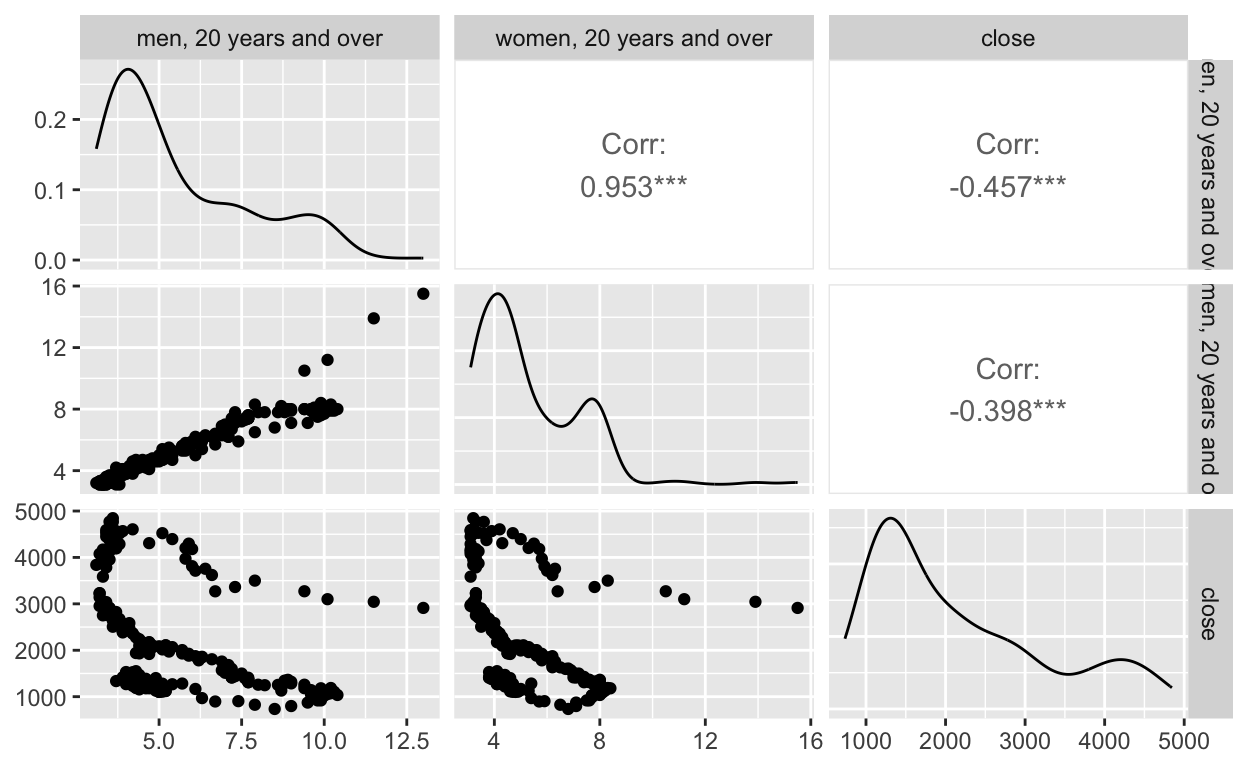
\includegraphics{Unemployment---the-Stock-Market-copy_files/figure-latex/unnamed-chunk-4-1.pdf}

\begin{Shaded}
\begin{Highlighting}[]
\CommentTok{\# Visualizing White unemployment rate from 2004 using ggplot2}
\NormalTok{stockData }\SpecialCharTok{|\textgreater{}} 
  \FunctionTok{ggplot}\NormalTok{(}\FunctionTok{aes}\NormalTok{(}\AttributeTok{x =}\NormalTok{ date, }\AttributeTok{y =}\NormalTok{ white)) }\SpecialCharTok{+}
  \FunctionTok{geom\_col}\NormalTok{(}\AttributeTok{na.rm =} \ConstantTok{TRUE}\NormalTok{) }\SpecialCharTok{+} 
  \FunctionTok{theme\_minimal}\NormalTok{(}\AttributeTok{base\_size =} \DecValTok{3}\NormalTok{) }\SpecialCharTok{+}
  \FunctionTok{theme}\NormalTok{(}\AttributeTok{axis.text.x =} \FunctionTok{element\_text}\NormalTok{(}\AttributeTok{angle =} \DecValTok{90}\NormalTok{))}
\end{Highlighting}
\end{Shaded}

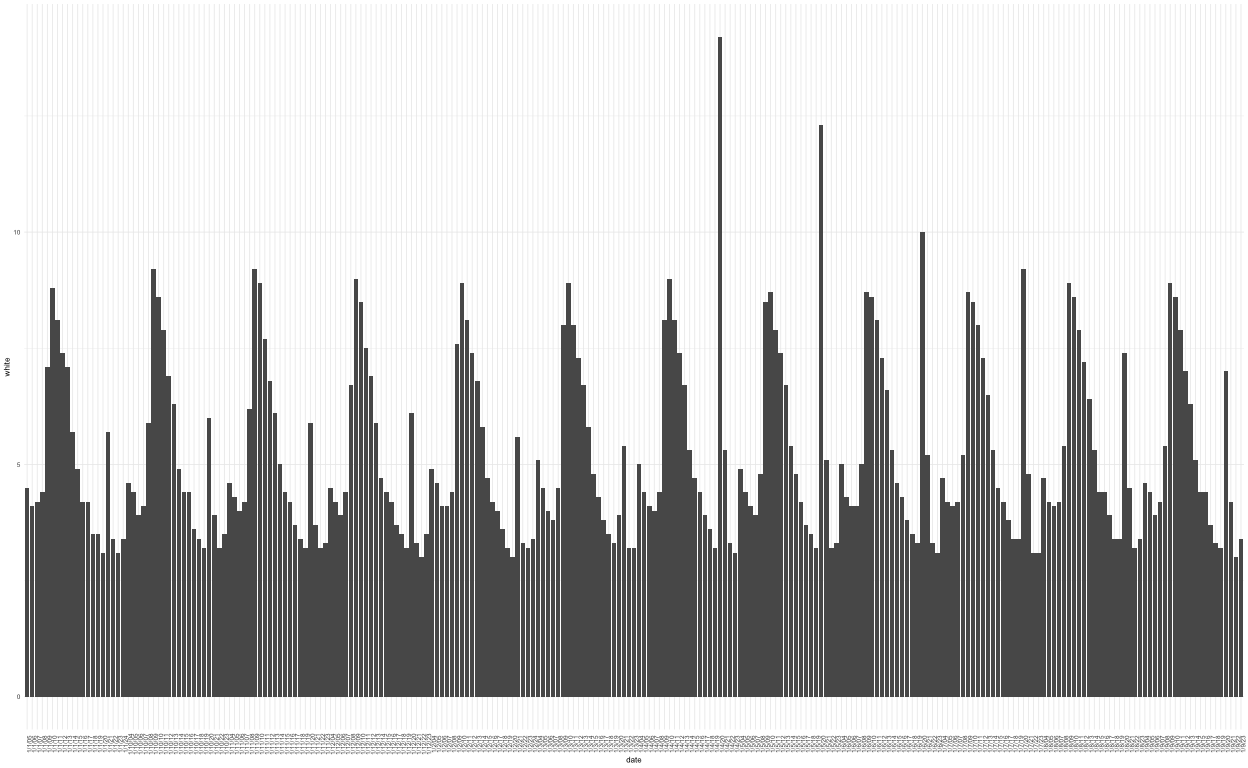
\includegraphics{Unemployment---the-Stock-Market-copy_files/figure-latex/unnamed-chunk-5-1.pdf}

\begin{Shaded}
\begin{Highlighting}[]
\CommentTok{\# Visualizing Hispanic unemployment rate from 2004 using ggplot2}
\NormalTok{stockData }\SpecialCharTok{|\textgreater{}}
  \FunctionTok{ggplot}\NormalTok{(}\FunctionTok{aes}\NormalTok{(}\AttributeTok{x =}\NormalTok{ date, }\AttributeTok{y =} \StringTok{\textasciigrave{}}\AttributeTok{hispanic or latino}\StringTok{\textasciigrave{}}\NormalTok{)) }\SpecialCharTok{+}
  \FunctionTok{geom\_col}\NormalTok{(}\AttributeTok{na.rm =} \ConstantTok{TRUE}\NormalTok{) }\SpecialCharTok{+} 
  \FunctionTok{theme\_minimal}\NormalTok{(}\AttributeTok{base\_size =} \DecValTok{3}\NormalTok{) }\SpecialCharTok{+}
  \FunctionTok{theme}\NormalTok{(}\AttributeTok{axis.text.x =} \FunctionTok{element\_text}\NormalTok{(}\AttributeTok{angle =} \DecValTok{90}\NormalTok{))}
\end{Highlighting}
\end{Shaded}

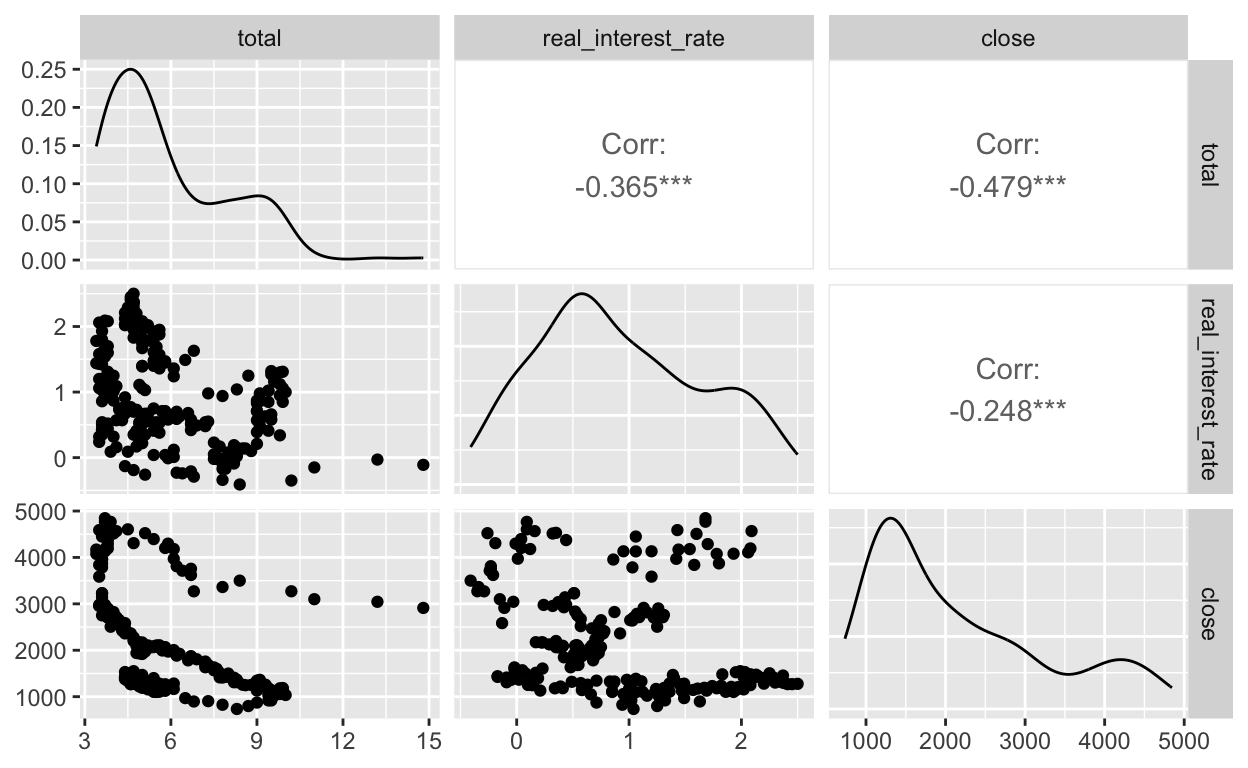
\includegraphics{Unemployment---the-Stock-Market-copy_files/figure-latex/unnamed-chunk-6-1.pdf}
From the three ethnic variables within the data, \texttt{white} and
\texttt{hispanic\ or\ latino} are similar in their distribution whereas
\texttt{black\ or\ african\ american} has a unique distribution.
However, there is a trend with all three graphs and that's they are
multimodial. In addition, the graph that shows the distribution of
unemployment amongst African Americans shows more significant peaks than
the other two graphs.

\begin{Shaded}
\begin{Highlighting}[]
\CommentTok{\# Visualizing the S\&P 500 trend from 2004 using ggplot2}
\FunctionTok{ggplot}\NormalTok{(stockData, }\FunctionTok{aes}\NormalTok{(}\AttributeTok{x =}\NormalTok{ date, }\AttributeTok{y =}\NormalTok{ close)) }\SpecialCharTok{+}
  \FunctionTok{geom\_col}\NormalTok{(}\AttributeTok{na.rm =} \ConstantTok{TRUE}\NormalTok{) }\SpecialCharTok{+} 
  \FunctionTok{theme\_minimal}\NormalTok{(}\AttributeTok{base\_size =} \DecValTok{3}\NormalTok{) }\SpecialCharTok{+}
  \FunctionTok{theme}\NormalTok{(}\AttributeTok{axis.text.x =} \FunctionTok{element\_text}\NormalTok{(}\AttributeTok{angle =} \DecValTok{90}\NormalTok{))}
\end{Highlighting}
\end{Shaded}

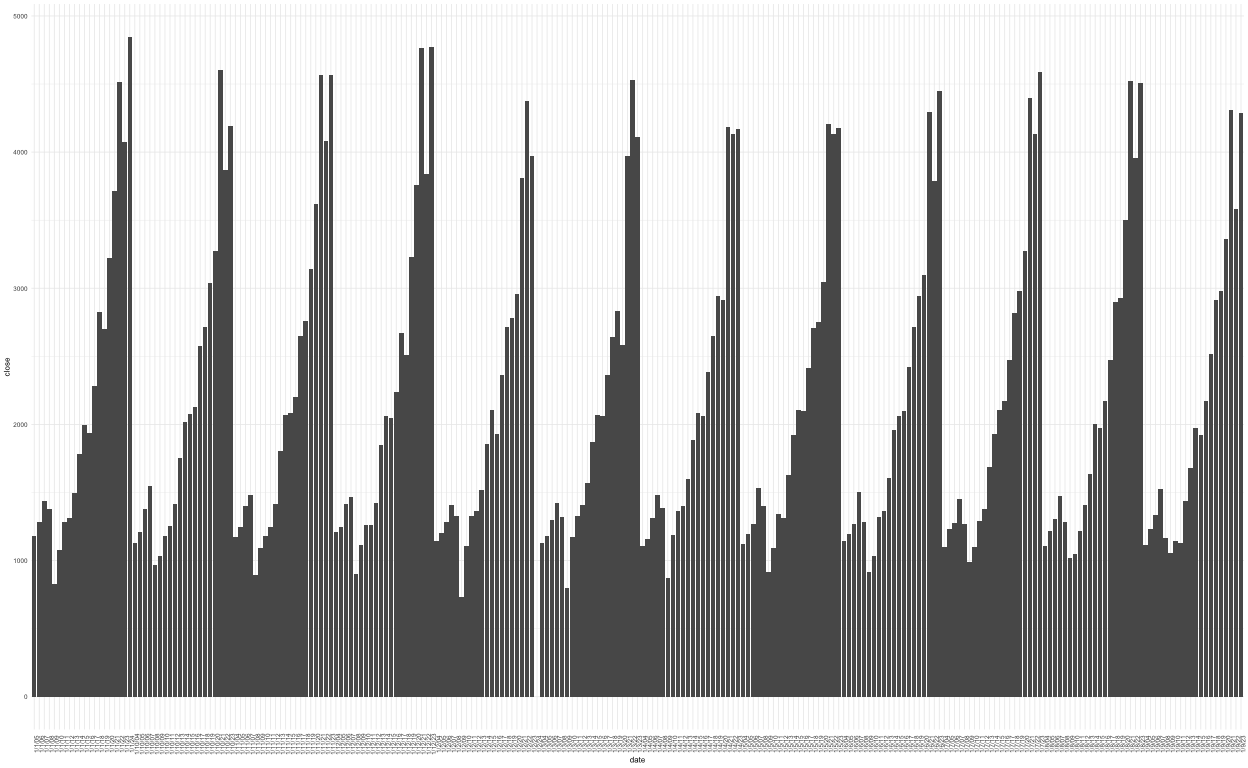
\includegraphics{Unemployment---the-Stock-Market-copy_files/figure-latex/unnamed-chunk-7-1.pdf}
As seen with the previous graphs, there closing prices of the S\&P 500
seem to be following a particular trend as well.

\textbf{Multiple Linear Regression}

When it comes to multiple linear regression, there are several
assumptions about the data. One of the most common ones is linear
relationship. we expected our data to have a linear relationship
(correlation), in other words, the closing price and the unemployment
rate need to move in a straight line whether negatively or positively.

Below are some graphs that visualize the relationship between the
closing price variable and other variables.

\textbf{Relationship between close price and the unemployment rate of
men and women over 20 years}

\begin{Shaded}
\begin{Highlighting}[]
\NormalTok{stockData }\SpecialCharTok{|\textgreater{}}
  \FunctionTok{select}\NormalTok{(}\StringTok{\textasciigrave{}}\AttributeTok{men, 20 years and over}\StringTok{\textasciigrave{}}\NormalTok{, }\StringTok{\textasciigrave{}}\AttributeTok{women, 20 years and over}\StringTok{\textasciigrave{}}\NormalTok{, close) }\SpecialCharTok{|\textgreater{}}
  \FunctionTok{ggpairs}\NormalTok{()}
\end{Highlighting}
\end{Shaded}

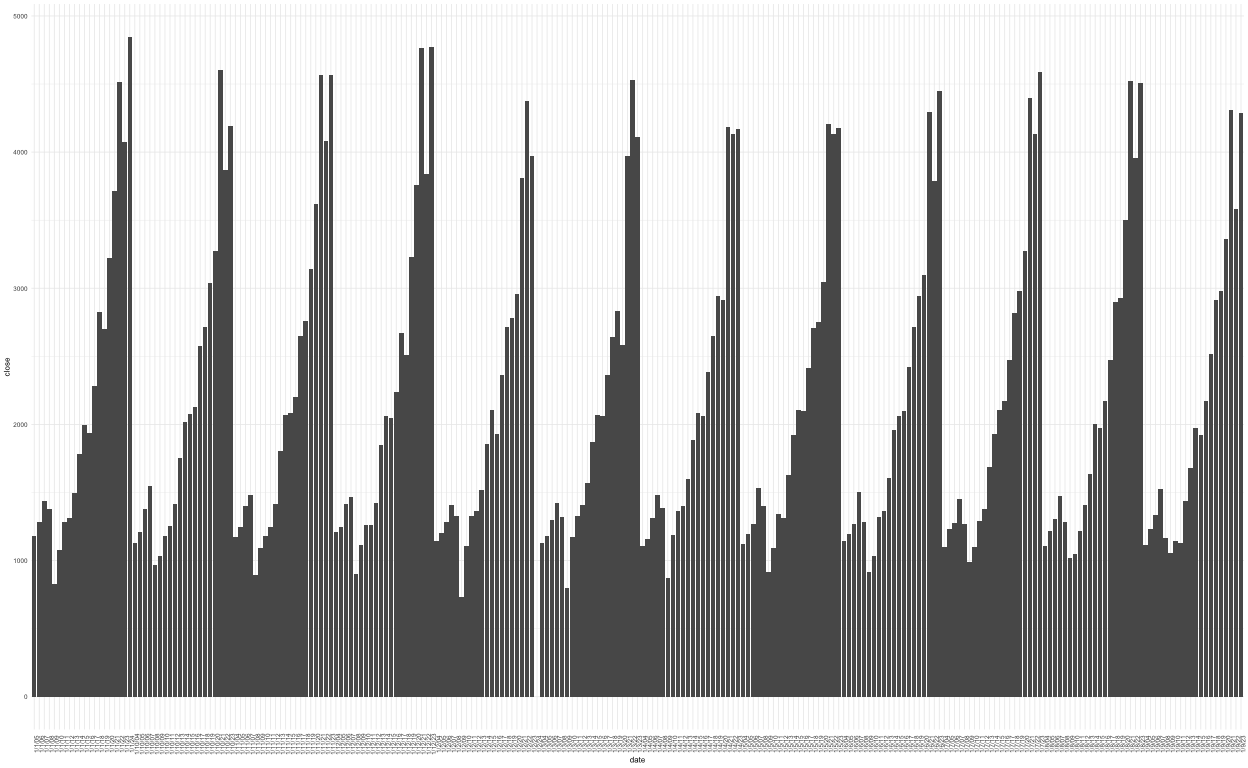
\includegraphics{Unemployment---the-Stock-Market-copy_files/figure-latex/unnamed-chunk-8-1.pdf}
Plot Results: As highlighted by the negative ``Corr:'' score, there is
negative correlation between the age variables with the close price
variable. In other words, when close price goes up, unemployment
decreases and vice versa when close prices goes down.

\textbf{Relationship between close price and the unemployment rate of
certain demographics}

\begin{Shaded}
\begin{Highlighting}[]
\NormalTok{stockData }\SpecialCharTok{|\textgreater{}}
  \FunctionTok{select}\NormalTok{(white, }\StringTok{\textasciigrave{}}\AttributeTok{black or african american}\StringTok{\textasciigrave{}}\NormalTok{, close) }\SpecialCharTok{|\textgreater{}}
  \FunctionTok{ggpairs}\NormalTok{()}
\end{Highlighting}
\end{Shaded}

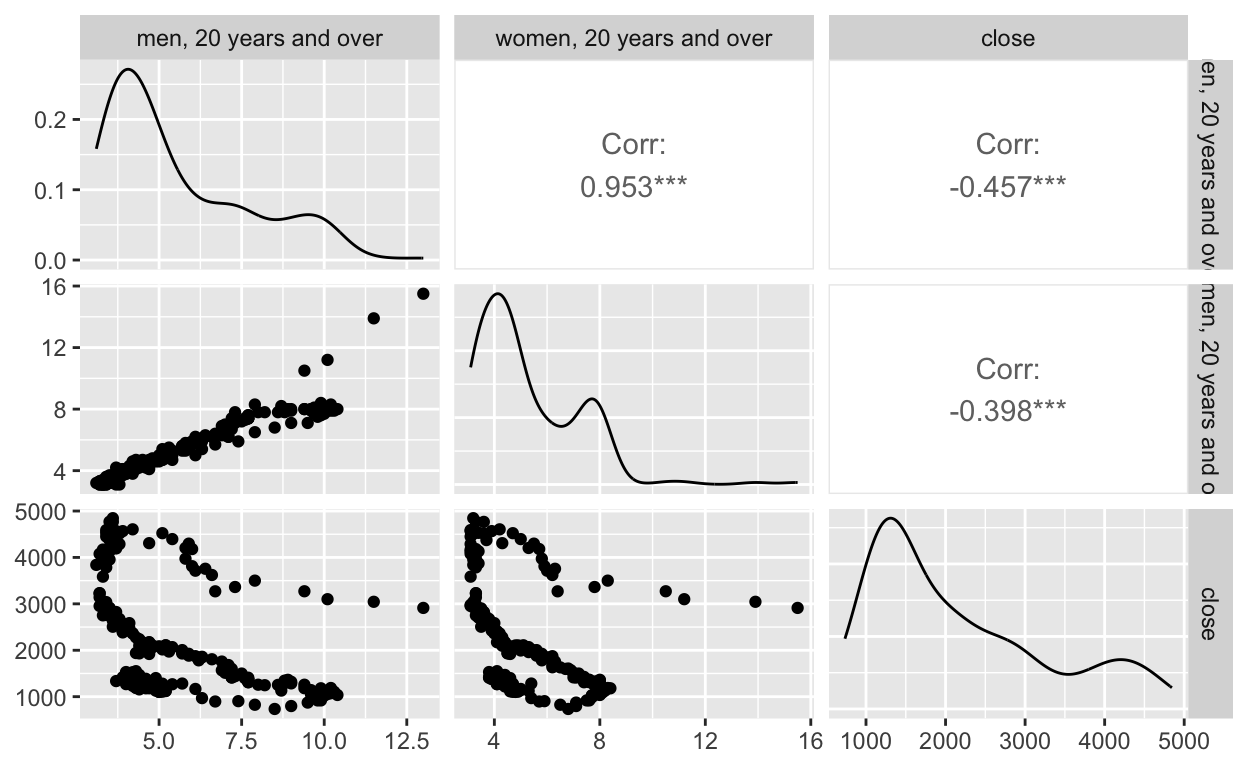
\includegraphics{Unemployment---the-Stock-Market-copy_files/figure-latex/unnamed-chunk-9-1.pdf}
Plot Results: As highlighted by the negative ``Corr:'' score, there is
negative correlation between the demographics variables with the close
price variable. In other words, although not definitive, when close
price goes up, unemployment for both White Americans and African
Americans decreases and vice versa when close prices goes down.

\textbf{Relationship between close price and total unemployment and real
interest rate}

\begin{Shaded}
\begin{Highlighting}[]
\NormalTok{stockData }\SpecialCharTok{|\textgreater{}}
  \FunctionTok{select}\NormalTok{(total, real\_interest\_rate, close) }\SpecialCharTok{|\textgreater{}}
  \FunctionTok{ggpairs}\NormalTok{()}
\end{Highlighting}
\end{Shaded}

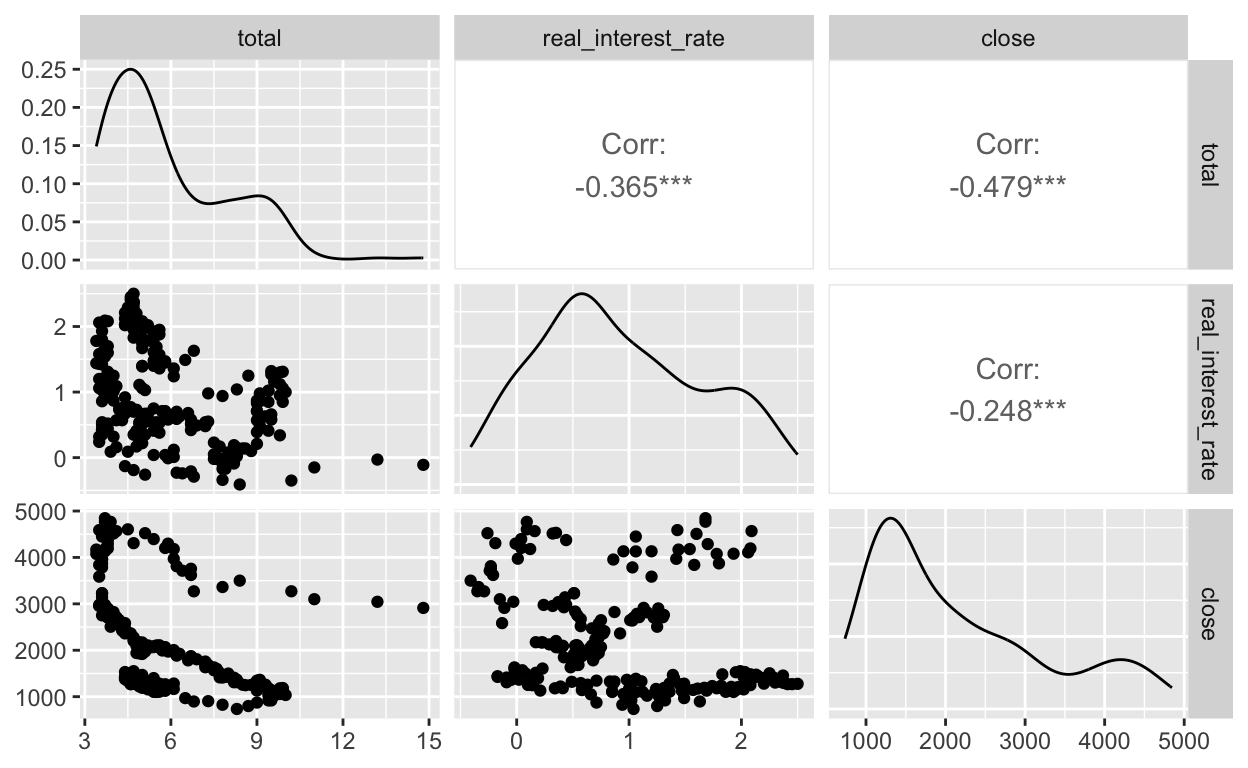
\includegraphics{Unemployment---the-Stock-Market-copy_files/figure-latex/unnamed-chunk-10-1.pdf}
Plot Results: As highlighted by the negative ``Corr:'' score, there is
negative correlation between the dependent variables with the close
price variable.

\textbf{Example}

To highlight the negative correlation, the plot below has a line that
shows how the points are plotted on the graph, highlighting how there is
negative correction.

\begin{Shaded}
\begin{Highlighting}[]
\NormalTok{stockData }\SpecialCharTok{|\textgreater{}}
  \FunctionTok{ggplot}\NormalTok{(}\FunctionTok{aes}\NormalTok{(close, }\AttributeTok{y =}\NormalTok{ white)) }\SpecialCharTok{+}
  \FunctionTok{geom\_point}\NormalTok{(}\AttributeTok{na.rm =} \ConstantTok{TRUE}\NormalTok{) }\SpecialCharTok{+}
  \FunctionTok{geom\_smooth}\NormalTok{(}\AttributeTok{method=}\NormalTok{lm, }\AttributeTok{se=}\ConstantTok{FALSE}\NormalTok{)}
\end{Highlighting}
\end{Shaded}

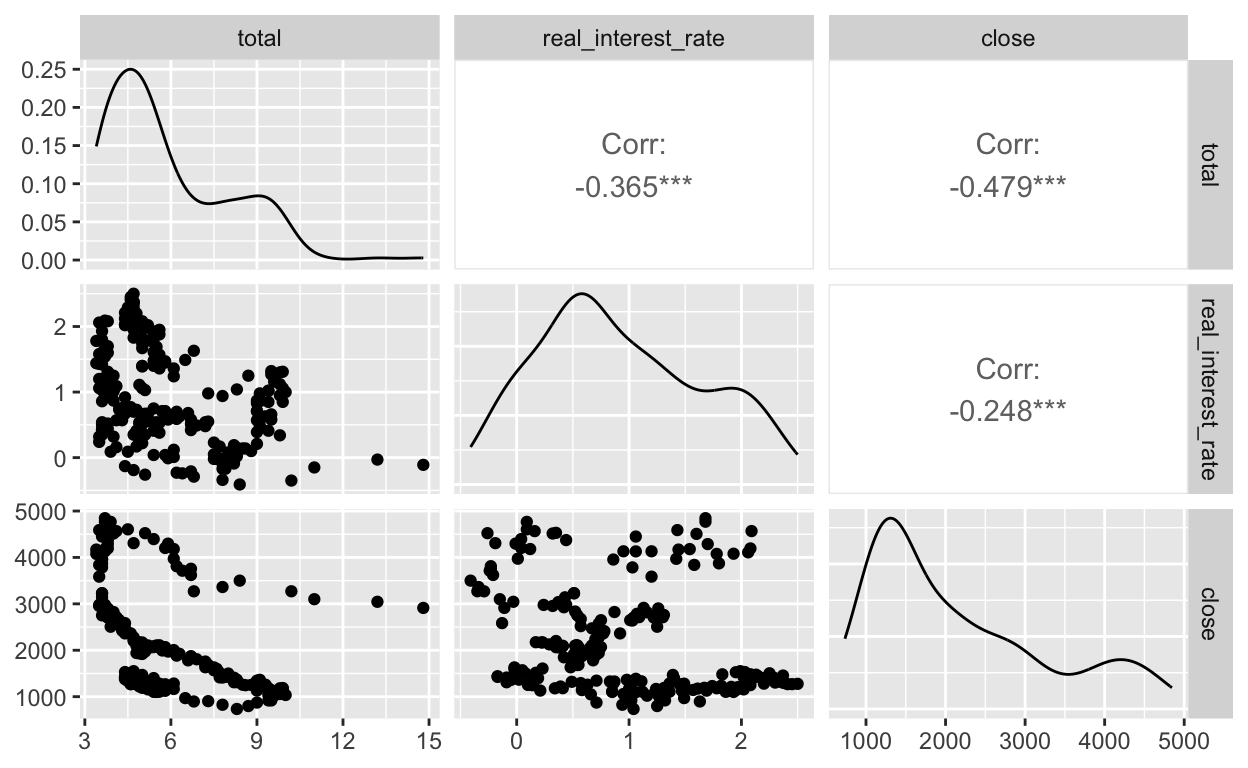
\includegraphics{Unemployment---the-Stock-Market-copy_files/figure-latex/unnamed-chunk-11-1.pdf}

\begin{Shaded}
\begin{Highlighting}[]
\NormalTok{stockData }\SpecialCharTok{|\textgreater{}}
  \FunctionTok{ggplot}\NormalTok{(}\FunctionTok{aes}\NormalTok{(close, }\AttributeTok{y =} \StringTok{\textasciigrave{}}\AttributeTok{black or african american}\StringTok{\textasciigrave{}}\NormalTok{)) }\SpecialCharTok{+}
  \FunctionTok{geom\_point}\NormalTok{(}\AttributeTok{na.rm =} \ConstantTok{TRUE}\NormalTok{) }\SpecialCharTok{+}
  \FunctionTok{geom\_smooth}\NormalTok{(}\AttributeTok{method=}\NormalTok{lm, }\AttributeTok{se=}\ConstantTok{FALSE}\NormalTok{)}
\end{Highlighting}
\end{Shaded}

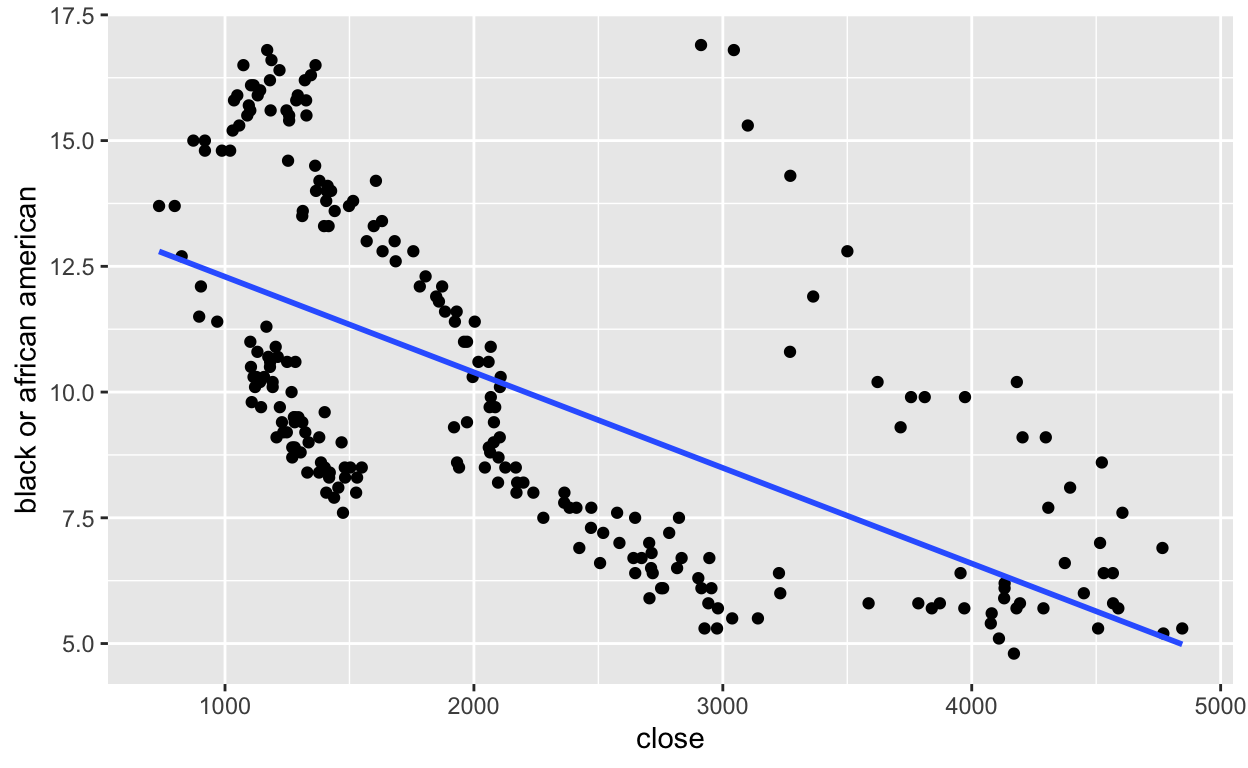
\includegraphics{Unemployment---the-Stock-Market-copy_files/figure-latex/unnamed-chunk-12-1.pdf}
\#\# Calculating the correlation

Another way we can calculate the correlation between vectors or
variables is by using the \texttt{cor()} function which serves the same
purpose as the graphs/plots above.

\begin{Shaded}
\begin{Highlighting}[]
\NormalTok{stockData }\SpecialCharTok{|\textgreater{}}
  \FunctionTok{na.omit}\NormalTok{() }\SpecialCharTok{|\textgreater{}}
  \FunctionTok{with}\NormalTok{(}\FunctionTok{cor}\NormalTok{(close, total))}
\end{Highlighting}
\end{Shaded}

\begin{verbatim}
## [1] -0.4788138
\end{verbatim}

\begin{Shaded}
\begin{Highlighting}[]
\NormalTok{stockData }\SpecialCharTok{|\textgreater{}}
  \FunctionTok{na.omit}\NormalTok{() }\SpecialCharTok{|\textgreater{}}
  \FunctionTok{with}\NormalTok{(}\FunctionTok{cor}\NormalTok{(close, }\StringTok{\textasciigrave{}}\AttributeTok{black or african american}\StringTok{\textasciigrave{}}\NormalTok{))}
\end{Highlighting}
\end{Shaded}

\begin{verbatim}
## [1] -0.6287374
\end{verbatim}

\begin{Shaded}
\begin{Highlighting}[]
\NormalTok{stockData }\SpecialCharTok{|\textgreater{}}
  \FunctionTok{na.omit}\NormalTok{() }\SpecialCharTok{|\textgreater{}}
  \FunctionTok{with}\NormalTok{(}\FunctionTok{cor}\NormalTok{(close, white))}
\end{Highlighting}
\end{Shaded}

\begin{verbatim}
## [1] -0.4602143
\end{verbatim}

\hypertarget{creating-multiple-linear-model}{%
\subsection{Creating Multiple Linear
Model}\label{creating-multiple-linear-model}}

\textbf{Determine and apply the appropriate generalized linear model for
a specific data context}

For this analysis, I am interested to see if there are specific factors
(mentioned at the beginning of this report) that affect the close price
of the S\&P 500. Since unemployment can be broken up by different
demographics including age and ethnicity, I will mainly focus on
enthnicity to see whether we need a multiple linear model or a single
linear model.

\textbf{Using \texttt{parsnip} to create specific linear model}

\begin{Shaded}
\begin{Highlighting}[]
\FunctionTok{library}\NormalTok{(parsnip)}

\CommentTok{\# Setting the mode to regression and engine to linear model}
\NormalTok{lm\_spec }\OtherTok{\textless{}{-}} \FunctionTok{linear\_reg}\NormalTok{() }\SpecialCharTok{\%\textgreater{}\%}
  \FunctionTok{set\_mode}\NormalTok{(}\StringTok{"regression"}\NormalTok{) }\SpecialCharTok{\%\textgreater{}\%}
  \FunctionTok{set\_engine}\NormalTok{(}\StringTok{"lm"}\NormalTok{)}

\NormalTok{lm\_spec}
\end{Highlighting}
\end{Shaded}

\begin{verbatim}
## Linear Regression Model Specification (regression)
## 
## Computational engine: lm
\end{verbatim}

\hypertarget{models}{%
\subsection{Models}\label{models}}

\emph{Use programming software (i.e., R) to fit and assess statistical
models}

\textbf{This multiple linear model (mlr) will look at \texttt{total}
unemployment and \texttt{real\_interest\_rate}}

\begin{Shaded}
\begin{Highlighting}[]
\NormalTok{mlr\_mod\_tot }\OtherTok{\textless{}{-}}\NormalTok{ lm\_spec }\SpecialCharTok{\%\textgreater{}\%} 
  \FunctionTok{fit}\NormalTok{(close }\SpecialCharTok{\textasciitilde{}}\NormalTok{ total }\SpecialCharTok{+}\NormalTok{ real\_interest\_rate, }\AttributeTok{data =}\NormalTok{ stockData)}

\FunctionTok{tidy}\NormalTok{(mlr\_mod\_tot)}
\end{Highlighting}
\end{Shaded}

\begin{verbatim}
## # A tibble: 3 x 5
##   term               estimate std.error statistic  p.value
##   <chr>                 <dbl>     <dbl>     <dbl>    <dbl>
## 1 (Intercept)           4867.     208.      23.5  1.07e-63
## 2 total                 -344.      27.4    -12.5  5.92e-28
## 3 real_interest_rate    -739.      79.5     -9.29 1.00e-17
\end{verbatim}

Results: If \texttt{total} or \texttt{real\_interest\_rate} are at 0
then the mean close would be 4867 (intercept estimate). In addition, for
every 1 unit increase in \texttt{total}, \texttt{close} will decrease by
-343.69; whereas a 1 unit increase in \texttt{total} will decrease
\texttt{close} by -738.8.

\textbf{This model will look at the age variables.}

\begin{Shaded}
\begin{Highlighting}[]
\NormalTok{mlr\_mod\_age }\OtherTok{\textless{}{-}}\NormalTok{ lm\_spec }\SpecialCharTok{\%\textgreater{}\%} 
  \FunctionTok{fit}\NormalTok{(close }\SpecialCharTok{\textasciitilde{}} \StringTok{\textasciigrave{}}\AttributeTok{men, 20 years and over}\StringTok{\textasciigrave{}} \SpecialCharTok{+} \StringTok{\textasciigrave{}}\AttributeTok{women, 20 years and over}\StringTok{\textasciigrave{}} \SpecialCharTok{+} \StringTok{\textasciigrave{}}\AttributeTok{16 to 19 years old}\StringTok{\textasciigrave{}}\NormalTok{, }\AttributeTok{data =}\NormalTok{ stockData)}

\FunctionTok{tidy}\NormalTok{(mlr\_mod\_age)}
\end{Highlighting}
\end{Shaded}

\begin{verbatim}
## # A tibble: 4 x 5
##   term                       estimate std.error statistic  p.value
##   <chr>                         <dbl>     <dbl>     <dbl>    <dbl>
## 1 (Intercept)                   5222.     162.      32.2  2.44e-88
## 2 `men, 20 years and over`       151.      70.7      2.14 3.32e- 2
## 3 `women, 20 years and over`     400.      72.2      5.54 8.21e- 8
## 4 `16 to 19 years old`          -345.      19.4    -17.8  1.35e-45
\end{verbatim}

Results: If \texttt{men,\ 20\ years\ and\ over},
\texttt{women,\ 20\ years\ and\ over} or \texttt{16\ to\ 19\ years\ old}
are at 0 then the mean close would be 5222.2 (intercept estimate).

For 1 unit increase in \texttt{men,\ 20\ years\ and\ over},
\texttt{close} will increase by 151.4 For 1 unit increase in
\texttt{women,\ 20\ years\ and\ over}, \texttt{close} will increase by
399.96 For 1 unit increase in \texttt{16\ to\ 19\ years\ old},
\texttt{close} will decrease by -344.9

\textbf{This model will look at the ethnicity variables.}

\begin{Shaded}
\begin{Highlighting}[]
\NormalTok{mlr\_mod\_demo }\OtherTok{\textless{}{-}}\NormalTok{ lm\_spec }\SpecialCharTok{\%\textgreater{}\%} 
  \FunctionTok{fit}\NormalTok{(close }\SpecialCharTok{\textasciitilde{}}\NormalTok{ white }\SpecialCharTok{+} \StringTok{\textasciigrave{}}\AttributeTok{black or african american}\StringTok{\textasciigrave{}} \SpecialCharTok{+} \StringTok{\textasciigrave{}}\AttributeTok{hispanic or latino}\StringTok{\textasciigrave{}}\NormalTok{, }\AttributeTok{data =}\NormalTok{ stockData)}

\FunctionTok{tidy}\NormalTok{(mlr\_mod\_demo)}
\end{Highlighting}
\end{Shaded}

\begin{verbatim}
## # A tibble: 4 x 5
##   term                        estimate std.error statistic  p.value
##   <chr>                          <dbl>     <dbl>     <dbl>    <dbl>
## 1 (Intercept)                   4669.      163.     28.6   1.52e-78
## 2 white                           72.2     220.      0.329 7.42e- 1
## 3 `black or african american`   -605.       43.1   -14.0   6.39e-33
## 4 `hispanic or latino`           438.      150.      2.93  3.74e- 3
\end{verbatim}

Results: If \texttt{white}, \texttt{black\ or\ african\ american} or
\texttt{hispanic\ or\ latino} are at 0 then the mean close would be
4668.84 (intercept estimate).

For 1 unit increase in \texttt{white}, \texttt{close} will increase by
72.2 For 1 unit increase in \texttt{black\ or\ african\ american},
\texttt{close} will decrease by -605.07 For 1 unit increase in
\texttt{hispanic\ or\ latino}, \texttt{close} will increase by 438.44

\textbf{This model excludes the \texttt{hispanic\ or\ latino} variable.}

\begin{Shaded}
\begin{Highlighting}[]
\NormalTok{mlr\_Wh\_Bl }\OtherTok{\textless{}{-}}\NormalTok{ lm\_spec }\SpecialCharTok{\%\textgreater{}\%} 
  \FunctionTok{fit}\NormalTok{(close }\SpecialCharTok{\textasciitilde{}}\NormalTok{ white }\SpecialCharTok{+} \StringTok{\textasciigrave{}}\AttributeTok{black or african american}\StringTok{\textasciigrave{}}\NormalTok{, }\AttributeTok{data =}\NormalTok{ stockData)}

\FunctionTok{tidy}\NormalTok{(mlr\_Wh\_Bl)}
\end{Highlighting}
\end{Shaded}

\begin{verbatim}
## # A tibble: 3 x 5
##   term                        estimate std.error statistic  p.value
##   <chr>                          <dbl>     <dbl>     <dbl>    <dbl>
## 1 (Intercept)                    4493.     154.      29.1  3.50e-80
## 2 white                           679.      73.7      9.21 1.73e-17
## 3 `black or african american`    -583.      43.1    -13.5  3.11e-31
\end{verbatim}

If \texttt{white} or \texttt{black\ or\ african\ american} are at 0 then
the mean close would be 4492.86 (intercept estimate).

For 1 unit increase in \texttt{white}, \texttt{close} will increase by
679.0 For 1 unit increase in \texttt{black\ or\ african\ american},
\texttt{close} will decrease by -582.84

\hypertarget{glance-at-models}{%
\subsection{Glance at models}\label{glance-at-models}}

To assess the goodness of fit of our models, we use the
\texttt{glance()} function. Basically, this function tell us how good
our model is by giving the model a ``score.'' Unfortunately, there is no
ideal ``score'' but the closer we get to one the better our model. Below
I shall interpret the results of each model by looking at the r.squared
value.

\begin{Shaded}
\begin{Highlighting}[]
\FunctionTok{glance}\NormalTok{(mlr\_mod\_tot)}
\end{Highlighting}
\end{Shaded}

\begin{verbatim}
## # A tibble: 1 x 12
##   r.squared adj.r.squared sigma statistic  p.value    df logLik   AIC   BIC
##       <dbl>         <dbl> <dbl>     <dbl>    <dbl> <dbl>  <dbl> <dbl> <dbl>
## 1     0.435         0.430  832.      91.3 4.02e-30     2 -1953. 3914. 3928.
## # i 3 more variables: deviance <dbl>, df.residual <int>, nobs <int>
\end{verbatim}

Results: This model looks at total unemployment rate and real interest
rate. Looking at the r.squared value, it is hard to say this is a good
model.

\begin{Shaded}
\begin{Highlighting}[]
\FunctionTok{glance}\NormalTok{(mlr\_mod\_age)}
\end{Highlighting}
\end{Shaded}

\begin{verbatim}
## # A tibble: 1 x 12
##   r.squared adj.r.squared sigma statistic  p.value    df logLik   AIC   BIC
##       <dbl>         <dbl> <dbl>     <dbl>    <dbl> <dbl>  <dbl> <dbl> <dbl>
## 1     0.670         0.665  638.      159. 1.80e-56     3 -1888. 3787. 3804.
## # i 3 more variables: deviance <dbl>, df.residual <int>, nobs <int>
\end{verbatim}

Results: This model is built using at the age variables and it seems to
perform better that the model

Below are the results I am most interested in. Interestingly, the model
that included the \texttt{Hispanic\ or\ Latino} ethnicity has a better
r.squared result as compared to the model that excluded that ethnicity.

\begin{Shaded}
\begin{Highlighting}[]
\FunctionTok{glance}\NormalTok{(mlr\_mod\_demo)}
\end{Highlighting}
\end{Shaded}

\begin{verbatim}
## # A tibble: 1 x 12
##   r.squared adj.r.squared sigma statistic  p.value    df logLik   AIC   BIC
##       <dbl>         <dbl> <dbl>     <dbl>    <dbl> <dbl>  <dbl> <dbl> <dbl>
## 1     0.570         0.565  727.      104. 4.66e-43     3 -1920. 3850. 3867.
## # i 3 more variables: deviance <dbl>, df.residual <int>, nobs <int>
\end{verbatim}

\begin{Shaded}
\begin{Highlighting}[]
\FunctionTok{glance}\NormalTok{(mlr\_Wh\_Bl)}
\end{Highlighting}
\end{Shaded}

\begin{verbatim}
## # A tibble: 1 x 12
##   r.squared adj.r.squared sigma statistic  p.value    df logLik   AIC   BIC
##       <dbl>         <dbl> <dbl>     <dbl>    <dbl> <dbl>  <dbl> <dbl> <dbl>
## 1     0.555         0.551  739.      148. 2.25e-42     2 -1924. 3856. 3870.
## # i 3 more variables: deviance <dbl>, df.residual <int>, nobs <int>
\end{verbatim}

Since the model above did not perform as well as I hoped they will, I
will go a step further and generated simple linear models for the
\texttt{white} ethnicity and the \texttt{black\ or\ african\ american}
ethnicity to see how they will perform individually.

\begin{Shaded}
\begin{Highlighting}[]
\NormalTok{lmr\_african }\OtherTok{\textless{}{-}}\NormalTok{ lm\_spec }\SpecialCharTok{\%\textgreater{}\%} 
  \FunctionTok{fit}\NormalTok{(close }\SpecialCharTok{\textasciitilde{}} \StringTok{\textasciigrave{}}\AttributeTok{black or african american}\StringTok{\textasciigrave{}}\NormalTok{, }\AttributeTok{data =}\NormalTok{ stockData)}

\FunctionTok{tidy}\NormalTok{(lmr\_african)}
\end{Highlighting}
\end{Shaded}

\begin{verbatim}
## # A tibble: 2 x 5
##   term                        estimate std.error statistic  p.value
##   <chr>                          <dbl>     <dbl>     <dbl>    <dbl>
## 1 (Intercept)                    4258.     177.       24.0 1.29e-65
## 2 `black or african american`    -208.      16.7     -12.5 8.21e-28
\end{verbatim}

\begin{Shaded}
\begin{Highlighting}[]
\FunctionTok{glance}\NormalTok{(lmr\_african)}
\end{Highlighting}
\end{Shaded}

\begin{verbatim}
## # A tibble: 1 x 12
##   r.squared adj.r.squared sigma statistic  p.value    df logLik   AIC   BIC
##       <dbl>         <dbl> <dbl>     <dbl>    <dbl> <dbl>  <dbl> <dbl> <dbl>
## 1     0.395         0.393  859.      156. 8.21e-28     1 -1961. 3928. 3938.
## # i 3 more variables: deviance <dbl>, df.residual <int>, nobs <int>
\end{verbatim}

\begin{Shaded}
\begin{Highlighting}[]
\NormalTok{lmr\_white }\OtherTok{\textless{}{-}}\NormalTok{ lm\_spec }\SpecialCharTok{\%\textgreater{}\%} 
  \FunctionTok{fit}\NormalTok{(close }\SpecialCharTok{\textasciitilde{}}\NormalTok{ white, }\AttributeTok{data =}\NormalTok{ stockData)}

\FunctionTok{tidy}\NormalTok{(lmr\_white)}
\end{Highlighting}
\end{Shaded}

\begin{verbatim}
## # A tibble: 2 x 5
##   term        estimate std.error statistic  p.value
##   <chr>          <dbl>     <dbl>     <dbl>    <dbl>
## 1 (Intercept)    3519.     181.      19.4  6.15e-51
## 2 white          -260.      32.5     -8.00 5.54e-14
\end{verbatim}

\begin{Shaded}
\begin{Highlighting}[]
\FunctionTok{glance}\NormalTok{(lmr\_white)}
\end{Highlighting}
\end{Shaded}

\begin{verbatim}
## # A tibble: 1 x 12
##   r.squared adj.r.squared sigma statistic  p.value    df logLik   AIC   BIC
##       <dbl>         <dbl> <dbl>     <dbl>    <dbl> <dbl>  <dbl> <dbl> <dbl>
## 1     0.212         0.208  981.      64.0 5.54e-14     1 -1993. 3992. 4002.
## # i 3 more variables: deviance <dbl>, df.residual <int>, nobs <int>
\end{verbatim}

Interestingly, both simple linear models have r.squared values that are
lower than the both the multiple linear models that preceded them.

\textbf{Conduct model selection for a set of candidate models}

\hypertarget{final-model}{%
\subsection{Final Model}\label{final-model}}

This part will aim to:

\begin{enumerate}
\def\labelenumi{\arabic{enumi}.}
\tightlist
\item
  Determine and apply the appropriate generalized linear model for a
  specific data context
\item
  Conduct model selection for a set of candidate models
\end{enumerate}

To choose my final model, I will work through the test/train process of
fitting and assessing the models.

\begin{Shaded}
\begin{Highlighting}[]
\CommentTok{\# Setting the seed}
\FunctionTok{set.seed}\NormalTok{(}\DecValTok{07}\NormalTok{)}

\CommentTok{\# Putting 80\% of the data into a training set}
\NormalTok{stockData\_split }\OtherTok{\textless{}{-}} \FunctionTok{initial\_split}\NormalTok{(stockData, }\AttributeTok{prop =} \FloatTok{0.80}\NormalTok{)}

\CommentTok{\# Assigning the two splits to data frames}
\NormalTok{stockData\_train }\OtherTok{\textless{}{-}} \FunctionTok{training}\NormalTok{(stockData\_split)}
\NormalTok{stockData\_test }\OtherTok{\textless{}{-}} \FunctionTok{testing}\NormalTok{(stockData\_split)}

\NormalTok{stockData\_train}
\end{Highlighting}
\end{Shaded}

\begin{verbatim}
## # A tibble: 192 x 16
##    date    total `men, 20 years and over` `women, 20 years and over`
##    <chr>   <dbl>                    <dbl>                      <dbl>
##  1 1/7/07    4.7                      4.2                        4.2
##  2 1/8/21    5.1                      5.1                        4.7
##  3 1/4/17    4.4                      3.9                        4.1
##  4 1/5/22    3.6                      3.4                        3.4
##  5 1/8/12    8.1                      7.6                        7.3
##  6 1/3/20    4.4                      4.1                        4  
##  7 1/4/05    5.2                      4.4                        4.6
##  8 1/3/22    3.6                      3.4                        3.4
##  9 1/11/13   6.9                      6.6                        6.2
## 10 1/5/15    5.6                      5.2                        5.1
## # i 182 more rows
## # i 12 more variables: `16 to 19 years old` <dbl>, white <dbl>,
## #   `black or african american` <dbl>, asian <dbl>, `hispanic or latino` <dbl>,
## #   open <dbl>, high <dbl>, low <dbl>, close <dbl>, `adj close` <dbl>,
## #   volume <dbl>, real_interest_rate <dbl>
\end{verbatim}

To choose a model between the different ethnic models I had, I decided
to go with the model that had the highest r.squared value which was the
model with all three ethnic variables. I made this decision because
everytime I removed a variable, the r.squared value kept on decreasing
(model performance was not improving).

\begin{Shaded}
\begin{Highlighting}[]
\NormalTok{mlr\_Traindemo }\OtherTok{\textless{}{-}}\NormalTok{ lm\_spec }\SpecialCharTok{\%\textgreater{}\%} 
  \FunctionTok{fit}\NormalTok{(close }\SpecialCharTok{\textasciitilde{}}\NormalTok{ white }\SpecialCharTok{+} \StringTok{\textasciigrave{}}\AttributeTok{black or african american}\StringTok{\textasciigrave{}} \SpecialCharTok{+} \StringTok{\textasciigrave{}}\AttributeTok{hispanic or latino}\StringTok{\textasciigrave{}}\NormalTok{, }\AttributeTok{data =}\NormalTok{ stockData\_train)}

\FunctionTok{tidy}\NormalTok{(mlr\_Traindemo)}
\end{Highlighting}
\end{Shaded}

\begin{verbatim}
## # A tibble: 4 x 5
##   term                        estimate std.error statistic  p.value
##   <chr>                          <dbl>     <dbl>     <dbl>    <dbl>
## 1 (Intercept)                   4566.      190.    24.0    3.02e-59
## 2 white                          -10.1     241.    -0.0419 9.67e- 1
## 3 `black or african american`   -575.       48.0  -12.0    6.49e-25
## 4 `hispanic or latino`           465.      168.     2.77   6.09e- 3
\end{verbatim}

\begin{Shaded}
\begin{Highlighting}[]
\FunctionTok{glance}\NormalTok{(mlr\_Traindemo)}
\end{Highlighting}
\end{Shaded}

\begin{verbatim}
## # A tibble: 1 x 12
##   r.squared adj.r.squared sigma statistic  p.value    df logLik   AIC   BIC
##       <dbl>         <dbl> <dbl>     <dbl>    <dbl> <dbl>  <dbl> <dbl> <dbl>
## 1     0.537         0.530  725.      72.7 2.86e-31     3 -1535. 3080. 3096.
## # i 3 more variables: deviance <dbl>, df.residual <int>, nobs <int>
\end{verbatim}

\begin{Shaded}
\begin{Highlighting}[]
\NormalTok{train\_aug }\OtherTok{\textless{}{-}} \FunctionTok{augment}\NormalTok{(mlr\_Traindemo, }\AttributeTok{new\_data =}\NormalTok{ stockData\_test)}
\NormalTok{train\_aug}
\end{Highlighting}
\end{Shaded}

\begin{verbatim}
## # A tibble: 49 x 18
##    .pred .resid date    total `men, 20 years and over` women, 20 years and ove~1
##    <dbl>  <dbl> <chr>   <dbl>                    <dbl>                     <dbl>
##  1 1725.  -584. 1/6/04    5.6                      5.1                       5  
##  2 1649.  -545. 1/8/04    5.4                      5                         4.7
##  3 1649.  -428. 1/8/05    4.9                      4.3                       4.4
##  4 2098.  -869. 1/9/05    5                        4.5                       4.6
##  5 1682.  -372. 1/4/06    4.7                      4.2                       4.3
##  6 2385.  -903. 1/11/07   4.7                      4.2                       4.2
##  7 2281.  -813. 1/12/07   5                        4.4                       4.4
##  8 2580. -1249. 1/2/08    4.9                      4.4                       4.2
##  9 2883. -1498. 1/4/08    5                        4.6                       4.2
## 10 2050. -1081. 1/10/08   6.5                      6.3                       5.4
## # i 39 more rows
## # i abbreviated name: 1: `women, 20 years and over`
## # i 12 more variables: `16 to 19 years old` <dbl>, white <dbl>,
## #   `black or african american` <dbl>, asian <dbl>, `hispanic or latino` <dbl>,
## #   open <dbl>, high <dbl>, low <dbl>, close <dbl>, `adj close` <dbl>,
## #   volume <dbl>, real_interest_rate <dbl>
\end{verbatim}

\textbf{Communicate the results of statistical models to a general
audience}

Results: Since the .resid (residual) values are negative, it means the
predicted value is too high. This result makes it difficult to justify
how accurate our model is. However, the plot below show random
distribution between the predicted values and the residuals which means
they are linear appropriate.

\begin{Shaded}
\begin{Highlighting}[]
\FunctionTok{ggplot}\NormalTok{(}\AttributeTok{data =}\NormalTok{ train\_aug, }\FunctionTok{aes}\NormalTok{(}\AttributeTok{x =}\NormalTok{ .pred, }\AttributeTok{y =}\NormalTok{ .resid)) }\SpecialCharTok{+}
  \FunctionTok{geom\_point}\NormalTok{() }\SpecialCharTok{+}
  \FunctionTok{geom\_hline}\NormalTok{(}\AttributeTok{yintercept =} \DecValTok{0}\NormalTok{, }\AttributeTok{linetype =} \StringTok{"dashed"}\NormalTok{, }\AttributeTok{color =} \StringTok{"red"}\NormalTok{) }\SpecialCharTok{+}
  \FunctionTok{xlab}\NormalTok{(}\StringTok{"Fitted values"}\NormalTok{) }\SpecialCharTok{+}
  \FunctionTok{ylab}\NormalTok{(}\StringTok{"Residuals"}\NormalTok{)}
\end{Highlighting}
\end{Shaded}

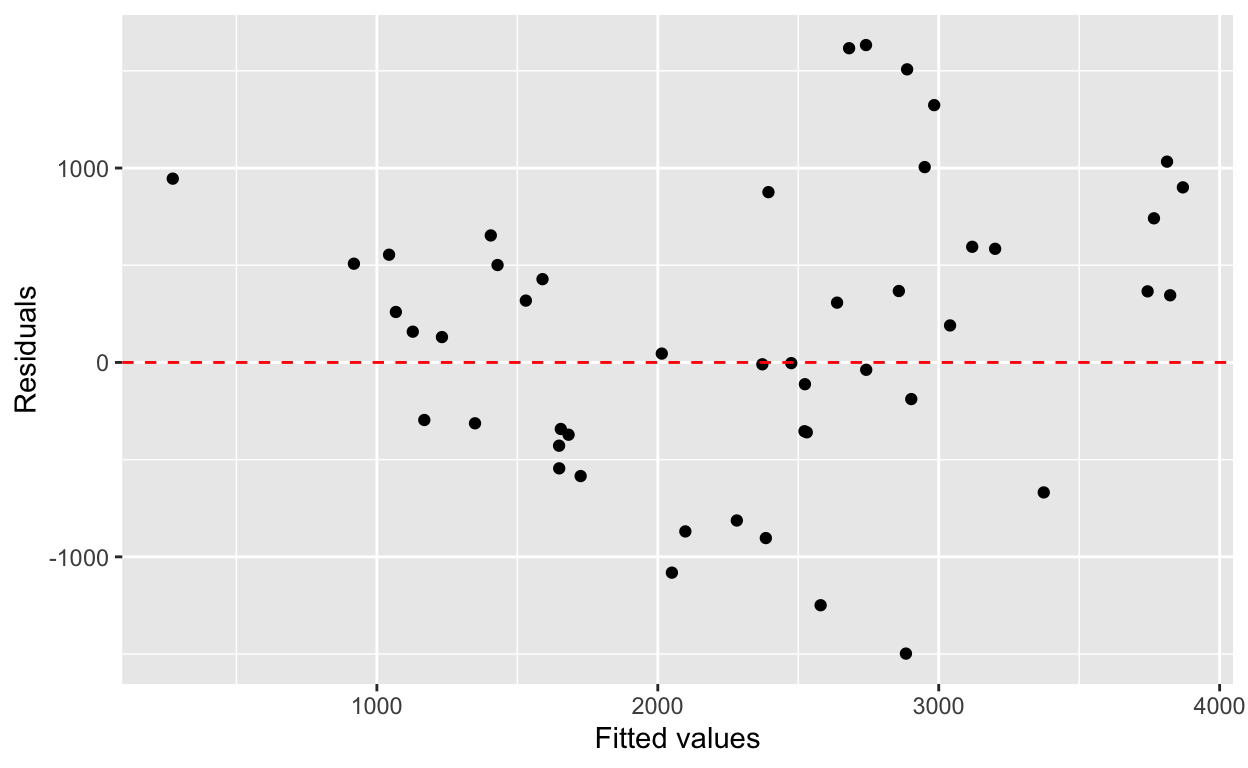
\includegraphics{Unemployment---the-Stock-Market-copy_files/figure-latex/fitted-residual-1.pdf}

\hypertarget{conclusion}{%
\subsection{Conclusion}\label{conclusion}}

In summation, there are a few things I can improve on which are
highlighted by this project. It was hard to state how accurate my model
was mainly due to the lack of data to create the model. My
\texttt{stockData} was over a 20 year period, which is not enough if we
want to have a good model. Without industry knowledge, it's hard to know
what a good r.squared value is hence I just went with the one closer to
1. In addition, I still need to work on how to interpret the results of
a test-train process. Overall, as I reflect on this process, I have
learned a lot more about models than I ever thought I could.

The goal of this analysis was to satisfy the following objectives and I
will state how I satisfied the objective:

\begin{enumerate}
\def\labelenumi{\arabic{enumi}.}
\item
  Describe probability as a foundation of statistical modeling,
  including inference and maximum likelihood estimation. I did this in
  the beginning of the \textbf{Analysis} section by defining what linear
  regression is. When it comes to modeling, the goal is to build a model
  that can predict a certain outcome. This prediction relies on
  probability which is derived from the historical data used to create
  the model.
\item
  Determine and apply the appropriate generalized linear model for a
  specific data context. Since unemployment can be broken up in various
  ways, I was curious to see how each ethnicity affects the stock
  prices. In this context, I ended up having both simple linear models
  and multiple linear models because the unemployment data was broken up
  into different demographics, hence I could build a model from one
  variable or multiple ones.
\item
  Conduct model selection for a set of candidate models. To perform
  this, I built different models and using the various demographic
  variables that I had along with total unemployment rate and interest
  rate. Once I had all the models, I used the \texttt{glance()} function
  to get the r.squared values of the models. From here I chose the
  ethnic model with the highest r.squared value because that is what I
  was interest in investigating.
\item
  Communicate the results of statistical models to a general audience. I
  communicated the results whenever I could. From talking about the
  distribution of the histograms to interpreting correlation results, I
  believed I was able to communicate results to a general audience.
\item
  Use programming software (i.e., R) to fit and assess statistical
  models. This was satisfied by this whole processes. By doing this
  project in R, I was able to use R to fit and assess statistical models
  using the test-train process and the \texttt{glance()} function as
  well.
\end{enumerate}

<!--radix_placeholder_site_after_body-->
<!--/radix_placeholder_site_after_body-->

<!--radix_placeholder_navigation_after_body-->
<!--/radix_placeholder_navigation_after_body-->

\end{document}
